
% !TeX root = dokumentation.tex

%!TEX root = ../dokumentation.tex
%
% Nahezu alle Einstellungen koennen hier getaetigt werden
%
\RequirePackage[l2tabu, orthodox]{nag}  % weist in Commandozeile bzw. log auf veraltete LaTeX Syntax hin
 
\documentclass[%
    pdftex,
    oneside,            % Einseitiger Druck.
    12pt,               % Schriftgroesse
    parskip=half,       % Halbe Zeile Abstand zwischen Absätzen.
%   topmargin = 10pt,   % Abstand Seitenrand (Std:1in) zu Kopfzeile [laut log: unused]
    headheight = 12pt,  % Höhe der Kopfzeile
%   headsep = 30pt, % Abstand zwischen Kopfzeile und Text Body  [laut log: unused]
    headsepline,        % Linie nach Kopfzeile.
    footsepline,        % Linie vor Fusszeile.
    footheight = 16pt,  % Höhe der Fusszeile
    abstracton,     % Abstract Überschriften
    DIV=calc,       % Satzspiegel berechnen
    BCOR=8mm,       % Bindekorrektur links: 8mm
    headinclude=false,  % Kopfzeile nicht in den Satzspiegel einbeziehen
    footinclude=false,  % Fußzeile nicht in den Satzspiegel einbeziehen
    listof=totoc,       % Abbildungs-/ Tabellenverzeichnis im Inhaltsverzeichnis darstellen
    toc=bibliography,   % Literaturverzeichnis im Inhaltsverzeichnis darstellen
]{scrreprt} % Koma-Script report-Klasse, fuer laengere Bachelorarbeiten alternativ auch: scrbook
 
% Einstellungen laden
\usepackage{xstring}
\usepackage[utf8]{inputenc}
\usepackage[T1]{fontenc}
 
\newcommand{\einstellung}[1]{%
  \expandafter\newcommand\csname #1\endcsname{}
  \expandafter\newcommand\csname setze#1\endcsname[1]{\expandafter\renewcommand\csname#1\endcsname{##1}}
}
\newcommand{\langstr}[1]{\einstellung{lang#1}}
 
\input{ads/einstellungen_liste} % verfügbare Einstellungen
%%%%%%%%%%%%%%%%%%%%%%%%%%%%%%%%%%%%%%%%%%%%%%%%%%%%%%%%%%%%%%%%%%%%%%%%%%%%%%%
%                                   Einstellungen
%
% Hier können alle relevanten Einstellungen für diese Arbeit gesetzt werden.
% Dazu gehören Angaben u.a. über den Autor sowie Formatierungen.
%
%
%%%%%%%%%%%%%%%%%%%%%%%%%%%%%%%%%%%%%%%%%%%%%%%%%%%%%%%%%%%%%%%%%%%%%%%%%%%%%%%


%%%%%%%%%%%%%%%%%%%%%%%%%%%%%%%%%%%% Sprache %%%%%%%%%%%%%%%%%%%%%%%%%%%%%%%%%%%
%% Aktuell sind Deutsch und Englisch unterstützt.
%% Es werden nicht nur alle vom Dokument erzeugten Texte in
%% der entsprechenden Sprache angezeigt, sondern auch weitere
%% Aspekte angepasst, wie z.B. die Anführungszeichen und
%% Datumsformate.
\setzesprache{de} % oder en
%%%%%%%%%%%%%%%%%%%%%%%%%%%%%%%%%%%%%%%%%%%%%%%%%%%%%%%%%%%%%%%%%%%%%%%%%%%%%%%%

%%%%%%%%%%%%%%%%%%%%%%%%%%%%%%%%%%% Angaben  %%%%%%%%%%%%%%%%%%%%%%%%%%%%%%%%%%%
%% Die meisten der folgenden Daten werden auf dem
%% Deckblatt angezeigt, einige auch im weiteren Verlauf
%% des Dokuments.
\setzematrikelnr{1695387}
\setzekurs{T41000}
\setzetitel{Evaluation und Implementierung einer robusten Netzwerkarchitektur zur Echtzeit-Übertragung von Sensordaten zwischen einem ESP32-Client und einem Raspberry Pi-basierten IoT-Stack}
\setzedatumAbgabe{07.09.2026}
\setzefirma{Mercedes-Benz AG}
\setzefirmenort{Stuttgart}
\setzeabgabeort{Stuttgart}
\setzeabschluss{T1000}
\setzestudiengang{Informatik}
\setzedhbw{Stuttgart}
\setzebetreuer{Paul Karcher B. Eng}
\setzegutachter{}
\setzezeitraum{01.10.2015 - 07.09.2026} % Hier kann man auch z.B. 12 Wochen als Zeitraum angeben
\setzearbeit{Projektarbeit}
\setzeautor{Viktoria Backhaus}
%%%%%%%%%%%%%%%%%%%%%%%%%%%%%%%%%%%%%%%%%%%%%%%%%%%%%%%%%%%%%%%%%%%%%%%%%%%%%%%%

%%%%%%%%%%%%%%%%%%%%%%%%%%%% Literaturverzeichnis %%%%%%%%%%%%%%%%%%%%%%%%%%%%%%
%% Bei Fehlern während der Verarbeitung bitte in ads/header.tex bei der
%% Einbindung des Pakets biblatex (ungefähr ab Zeile 110,
%% einmal für jede Sprache), biber in bibtex ändern.
\newcommand{\ladeliteratur}{%
%\addbibresource{bibliographie.bib}
\addbibresource{quellen.bib}
}
%% Zitierstil
%% siehe: http://ctan.mirrorcatalogs.com/macros/latex/contrib/biblatex/doc/biblatex.pdf (3.3.1 Citation Styles)
%% mögliche Werte z.B numeric-comp, alphabetic, authoryear
\setzezitierstil{numeric-comp}
%%%%%%%%%%%%%%%%%%%%%%%%%%%%%%%%%%%%%%%%%%%%%%%%%%%%%%%%%%%%%%%%%%%%%%%%%%%%%%%%

%%%%%%%%%%%%%%%%%%%%%%%%%%%%%%%%% Layout %%%%%%%%%%%%%%%%%%%%%%%%%%%%%%%%%%%%%%%
%% Verschiedene Schriftarten
% laut nag Warnung: palatino obsolete, use mathpazo, helvet (option scaled=.95), courier instead
\setzeschriftart{lmodern} % palatino oder goudysans, lmodern, libertine

%% Paket um Textteile drehen zu können
%\usepackage{rotating}
%% Paket um Seite im Querformat anzuzeigen
%\usepackage{lscape}

%% Seitenränder
\setzeseitenrand{2.5cm}

%% Abstand vor Kapitelüberschriften zum oberen Seitenrand
\setzekapitelabstand{20pt}

%% Spaltenabstand
\setzespaltenabstand{10pt}
%%Zeilenabstand innerhalb einer Tabelle
\setzezeilenabstand{1.5}
%%%%%%%%%%%%%%%%%%%%%%%%%%%%%%%%%%%%%%%%%%%%%%%%%%%%%%%%%%%%%%%%%%%%%%%%%%%%%%%%

%%%%%%%%%%%%%%%%%%%%%%%%%%%%% Verschiedenes  %%%%%%%%%%%%%%%%%%%%%%%%%%%%%%%%%%%
%% Farben (Angabe in HTML-Notation mit großen Buchstaben)
\newcommand{\ladefarben}{%
	\definecolor{LinkColor}{HTML}{000000} % war ursprünglich 00007A
	\definecolor{ListingBackground}{HTML}{FCF7DE}
}
%% Mathematikpakete benutzen (Pakete aktivieren)
%\usepackage{amsmath}
%\usepackage{amssymb}

%% Programmiersprachen Highlighting (Listings)
\newcommand{\listingsettings}{%
	\lstset{%
		language=Java,			% Standardsprache des Quellcodes
		numbers=left,			% Zeilennummern links
		stepnumber=1,			% Jede Zeile nummerieren.
		numbersep=5pt,			% 5pt Abstand zum Quellcode
		numberstyle=\tiny,		% Zeichengrösse 'tiny' für die Nummern.
		breaklines=true,		% Zeilen umbrechen wenn notwendig.
		breakautoindent=true,	% Nach dem Zeilenumbruch Zeile einrücken.
		postbreak=\space,		% Bei Leerzeichen umbrechen.
		tabsize=2,				% Tabulatorgrösse 2
		basicstyle=\ttfamily\footnotesize, % Nichtproportionale Schrift, klein für den Quellcode
		showspaces=false,		% Leerzeichen nicht anzeigen.
		showstringspaces=false,	% Leerzeichen auch in Strings ('') nicht anzeigen.
		extendedchars=true,		% Alle Zeichen vom Latin1 Zeichensatz anzeigen.
		captionpos=b,			% sets the caption-position to bottom
		backgroundcolor=\color{ListingBackground}, % Hintergrundfarbe des Quellcodes setzen.
		xleftmargin=0pt,		% Rand links
		xrightmargin=0pt,		% Rand rechts
		frame=single,			% Rahmen an
		frameround=ffff,
		rulecolor=\color{darkgray},	% Rahmenfarbe
		fillcolor=\color{ListingBackground},
		keywordstyle=\color[rgb]{0.133,0.133,0.6},
		commentstyle=\color[rgb]{0.133,0.545,0.133},
		stringstyle=\color[rgb]{0.627,0.126,0.941}
	}
}
%%%%%%%%%%%%%%%%%%%%%%%%%%%%%%%%%%%%%%%%%%%%%%%%%%%%%%%%%%%%%%%%%%%%%%%%%%%%%%%%

%%%%%%%%%%%%%%%%%%%%%%%%%%%%%%%% Eigenes %%%%%%%%%%%%%%%%%%%%%%%%%%%%%%%%%%%%%%%
%% Hier können Ergänzungen zur Präambel vorgenommen werden (eigene Pakete, Einstellungen)
%% custom Quellenangabe
\usepackage{xifthen}
% first: indirect or direct
% second: lecture
% third: startpage
% fourth: endpage
\newcommand{\citeM}[4]
{(\ifthenelse{\equal{#1}{i}}{vgl.~}{}\cite{#2}\ifthenelse{\equal{#3}{} \AND \equal{#4}{}}{}{\ifthenelse{\equal{#1}{c}}{,~Z.}{,~S.}\ifthenelse{\equal{#3}{#4}}{#3}{#3-#4}})}

\usepackage{tikz}
\usetikzlibrary{shapes.geometric, arrows}

\usepackage{smartdiagram}


 % lese Einstellungen
 
\input{lang/strings} % verfügbare Strings
\input{lang/\sprache} % Übersetzung einlesen
 
% Einstellung der Sprache des Paketes Babel und der Verzeichnisüberschriften
\iflang{de}{\usepackage[english, ngerman]{babel}}
\iflang{en}{\usepackage[ngerman, english]{babel}}
 
 
%%%%%%% Package Includes %%%%%%%
 
\usepackage[margin=\seitenrand,foot=1cm]{geometry}  % Seitenränder und Abstände
\usepackage[activate]{microtype} %Zeilenumbruch und mehr
\usepackage[onehalfspacing]{setspace}
\usepackage{makeidx}
\usepackage[autostyle=true,german=quotes]{csquotes}
\usepackage{longtable}
\usepackage{enumitem}   % mehr Optionen bei Aufzählungen
\usepackage{graphicx}
\usepackage{booktabs}
\usepackage{pdfpages}   % zum Einbinden von PDFs
\usepackage{xcolor}     % für HTML-Notation
\usepackage{float}
\usepackage{array}
\usepackage{calc}       % zum Rechnen (Bildtabelle in Deckblatt)
\usepackage[right]{eurosym}
\usepackage{wrapfig}
\usepackage{pgffor} % für automatische Kapiteldateieinbindung
\usepackage[perpage, hang, multiple, stable]{footmisc} % Fussnoten
\usepackage[printonlyused]{acronym} % falls gewünscht kann die Option footnote eingefügt werden, dann wird die Erklärung nicht inline sondern in einer Fußnote dargestellt
\usepackage{listings}
 
% Notizen. Einsatz mit \todo{Notiz} oder \todo[inline]{Notiz}.
\usepackage[obeyFinal,backgroundcolor=yellow,linecolor=black]{todonotes}
% Alle Notizen ausblenden mit der Option "final" in \documentclass[...] oder durch das auskommentieren folgender Zeile
% \usepackage[disable]{todonotes}
 
%%%%%%%%%%%%%%%
%own packages
\usepackage{pgfplots}
\usepackage{tikz}
\usepackage{subcaption}
\usetikzlibrary{shapes,arrows,calc,fit,backgrounds,shapes.multipart,math,angles,quotes,patterns}
\pgfplotsset{compat=1.18}
\usepackage{amsmath, amssymb}
\usepackage{interval}
\usepackage{struktex}
 
 
% Kommentarumgebung. Einsatz mit \comment{}. Alle Kommentare ausblenden mit dem Auskommentieren der folgenden und dem aktivieren der nächsten Zeile.
\newcommand{\comment}[1]{\par {\bfseries \color{blue} #1 \par}} %Kommentar anzeigen
% \newcommand{\comment}[1]{} %Kommentar ausblenden
 
 
%%%%%% Configuration %%%%%
 
%% Anwenden der Einstellungen
 
\usepackage{\schriftart}
\ladefarben{}
 
% Titel, Autor und Datum
\title{\titel}
\author{\autor}
\date{\datum}
 
% PDF Einstellungen
\usepackage[%
    pdftitle={\titel},
    pdfauthor={\autor},
    pdfsubject={\arbeit},
    pdfcreator={pdflatex, LaTeX with KOMA-Script},
    pdfpagemode=UseOutlines,        % Beim Oeffnen Inhaltsverzeichnis anzeigen
    pdfdisplaydoctitle=true,        % Dokumenttitel statt Dateiname anzeigen.
    pdflang={\sprache},             % Sprache des Dokuments.
]{hyperref}
 
% (Farb-)einstellungen für die Links im PDF
\hypersetup{%
    colorlinks=true,        % Aktivieren von farbigen Links im Dokument
    linkcolor=LinkColor,    % Farbe festlegen
    citecolor=LinkColor,
    filecolor=LinkColor,
    menucolor=LinkColor,
    urlcolor=LinkColor,
    linktoc=all,            % der komplette text eines Eintrages im Table of Contents wird klickbar
    linktocpage=false,      % Nicht der Text sondern die Seitenzahlen in Verzeichnissen klickbar wenn true, hab ich aber deaktiviert
    bookmarksnumbered=true  % Überschriftsnummerierung im PDF Inhalt anzeigen.
}
% Workaround um Fehler in Hyperref, muss hier stehen bleiben
\usepackage{bookmark} %nur ein latex-Durchlauf für die Aktualisierung von Verzeichnissen nötig
 
% Schriftart in Captions etwas kleiner
\addtokomafont{caption}{\small}
 
% Literaturverweise (sowohl deutsch als auch englisch)
\iflang{de}{%
\usepackage[
    backend=bibtex,     % empfohlen. Falls biber Probleme macht: bibtex
    bibwarn=true,
    bibencoding=utf8,   % wenn .bib in utf8, sonst ascii
    sortlocale=de_DE,
    style=\zitierstil,
]{biblatex}
\DeclareFieldFormat{urldate}{\mkbibparens{zuletzt geprüft\addcolon\space#1}}
\DeclareBibliographyDriver{online}{%
  \usebibmacro{bibindex}%
  \usebibmacro{begentry}%
  \usebibmacro{author/editor}%
  \setunit{\labelnamepunct}\newblock
  \usebibmacro{title}%
  \newunit\newblock
  \usebibmacro{byauthor}%
  \newunit\newblock
  \usebibmacro{byeditor+others}%
  \newunit\newblock
  \usebibmacro{date}%
  \newunit\newblock
  \usebibmacro{url}%
  \newunit\newblock%
  \printfield{note}%
  \newunit\newblock
  \usebibmacro{addendum+pubstate}%
  \usebibmacro{pageref}%
  \usebibmacro{finentry}}
}
\iflang{en}{%
\usepackage[
    backend=biber,      % empfohlen. Falls biber Probleme macht: bibtex
    bibwarn=true,
    bibencoding=utf8,   % wenn .bib in utf8, sonst ascii
    sortlocale=en_US,
    style=\zitierstil,
]{biblatex}
}
 
\ladeliteratur{}
 
% Glossar
\usepackage[nonumberlist,toc]{glossaries}
 
%%%%%% Additional settings %%%%%%
 
% Hurenkinder und Schusterjungen verhindern
% http://projekte.dante.de/DanteFAQ/Silbentrennung
\clubpenalty = 10000 % schließt Schusterjungen aus (Seitenumbruch nach der ersten Zeile eines neuen Absatzes)
\widowpenalty = 10000 % schließt Hurenkinder aus (die letzte Zeile eines Absatzes steht auf einer neuen Seite)
\displaywidowpenalty=10000
 
% Bildpfad
\graphicspath{{images/}}
 
% Einige häufig verwendete Sprachen
\lstloadlanguages{PHP,Python,Java,C,C++,bash}
\listingsettings{}
% Umbennung des Listings
\renewcommand\lstlistingname{\langlistingname}
\renewcommand\lstlistlistingname{\langlistlistingname}
\def\lstlistingautorefname{\langlistingautorefname}
 
% Abstände in Tabellen
\setlength{\tabcolsep}{\spaltenabstand}
\renewcommand{\arraystretch}{\zeilenabstand}
 
% speziell für Tabellen
\usepackage{tabularx}
\usepackage{longtable}
% left fixed width:
\newcolumntype{L}[1]{>{\raggedright\arraybackslash}m{#1}}

\makeglossaries
\input{ads/glossary}

\begin{document}

	% Deckblatt
	\begin{spacing}{1}
		\input{ads/deckblatt}
	\end{spacing}
	\newpage

	\pagenumbering{Roman}

	% Sperrvermerk
	\input{ads/sperrvermerk}
	\newpage

	% Erklärung
	\input{ads/erklaerung}
	\newpage

	% Abstract
	%\input{ads/abstract}
	%\newpage


    %========================================================
    %Hier je nach Bedarf für Gendererklärung / Danksagung einkommentieren
    
    %\input{ads/gendererklaerung}
    %\newpage
    
    %\input{ads/acknowledgement}
    %\newpage

    %=========================================================

	\pagestyle{plain}		% nur Seitenzahlen im Fuß
	
	\RedeclareSectionCommand[beforeskip=\kapitelabstand         ]{chapter} % stellt Abstand vor Kapitelüberschriften ein

	% Inhaltsverzeichnis
	\begin{spacing}{1.1}
		\begingroup
		
			% auskommentieren für Seitenzahlen unter Inhaltsverzeichnis
			\renewcommand*{\chapterpagestyle}{empty}
			\pagestyle{empty}
			
			
			\setcounter{tocdepth}{2}
			%für die Anzeige von Unterkapiteln im Inhaltsverzeichnis
			%\setcounter{tocdepth}{1}
			
			\tableofcontents
			\clearpage
		\endgroup
	\end{spacing}
	\newpage

	% Abkürzungsverzeichnis
	\cleardoublepage
	%!TEX root = ../dokumentation.tex

\addchap{\langabkverz}
%nur verwendete Akronyme werden letztlich im Abkürzungsverzeichnis des Dokuments angezeigt
%Verwendung: 
%		\ac{Abk.}   --> fügt die Abkürzung ein, beim ersten Aufruf wird zusätzlich automatisch die ausgeschriebene Version davor eingefügt bzw. in einer Fußnote (hierfür muss in header.tex \usepackage[printonlyused,footnote]{acronym} stehen) dargestellt
%		\acs{Abk.}   -->  fügt die Abkürzung ein
%		\acf{Abk.}   --> fügt die Abkürzung UND die Erklärung ein
%		\acl{Abk.}   --> fügt nur die Erklärung ein
%		\acp{Abk.}  --> gibt Plural aus (angefügtes 's'); das zusätzliche 'p' funktioniert auch bei obigen Befehlen
%       \aclp{Abk.} --> gibt die Erklärung in Plura (angefügtes 's' aus
%	siehe auch: http://golatex.de/wiki/%5Cacronym
%	
\begin{acronym}[YTMMM]
\setlength{\itemsep}{.5\parsep}

\acro{API}{App Programming Interface}
\acro{DHBW}{Duale Hochschule Baden-Würtemberg}
\acro{HVAC}{Heating, Ventilation and Air Conditioning}
\acro{MCU}{Mikrocontroller-Einheit}
\acro{EEPROM}{electrically erasable programmable read-only memory}
\acro{IoT}{Internet of Things}
\acro{OSI}{Open Systems Interconnection}
\acro{TCP}{Transmission Control Protocol}
\acro{UDP}{User Datagram Protocol}
\acro{IP}{Internet Protocol}
\acro{MAC}{Media Access Control}
\acro{ACK}{Acknowledgement}
\acro{CSMA/CD}{Carrier Sense Multiple Access with Collision Detection}
\acro{CSMA/CA}{Carrier Sense Multiple Access with Collision Avoidance}
\acro{MQTT}{Message Queuing Telemetry Transport}
\acro{HTTP}{Hypertext Transfer Protocol}
\acro{HTTPS}{Hypertext Transfer Protocol Secure}
\acro{DNS}{Domain Name System}
\end{acronym}


	% Abbildungsverzeichnis
	\cleardoublepage
	\listoffigures

	%Tabellenverzeichnis
	%\cleardoublepage
	%\listoftables

	% Quellcodeverzeichnis
	%\cleardoublepage
	%\lstlistoflistings

	% Formatierungen
	%\cleardoublepage
	%\input{ads/formatting.tex}
	\cleardoublepage

	\pagenumbering{arabic}
	
	\pagestyle{headings}		% Kolumnentitel im Kopf, Seitenzahlen im Fuß


    %Anleitung kann hier ausgeblendet werden, damit Kapitel 1 erst ab 01kapitel.tex anfängt
    %---------------------------------------------------------------------------------------
    %%!TEX root = ../dokumentation.tex
\chapter{Gebrauchsanleitung}

Bitte diese Anleitung durchlesen. \\

Um diese Anleitung in der eigentlichen Arbeit auszublenden, kommentieren Sie bitte die anleitung.tex (und das \textbackslash newpage) in der dokumentation.tex aus. \\
\textbf{Mit dem auskommentieren der Anleitung startet die Vorlage bei 01kapitel.tex (momentan Kapitel 4 'Einleitung').}

\section{Übersicht über die Vorlage}

\begin{table}[h!]
    \centering
    \begin{tabularx}{\textwidth}{lX}
        \textbf{Dateiname} & \textbf{Beschreibung} \\\toprule
        \texttt{dokumentation.tex} & Die Hauptdatei. Alle anderen Dateien werden von dieser Datei eingezogen. \textbf{Hier Hinzufügen / Löschen von Frontmatter!} \\
        \texttt{abstract.tex} & Die Kurzfassung der Arbeit. \\    
        \texttt{header.tex} & Konfigurationseinstellungen der einzelnen Pakete \\
        \texttt{acronyms.tex} & Definition von Abkürzungen. \\
        \texttt{acknowledgement.tex} & Danksagung (Für Bachelorarbeit) \\
        \texttt{deckblatt.tex} & Titelseite der Arbeit. \\
        \texttt{anleitung.tex} & Diese Anleitung \\ 
        \texttt{bibliography.bib bzw. quellen.bib} & Die Literaturdatenbank -- hier können Sie die verwendete Literatur einpflegen. Eine davon verwenden.\\
        \texttt{erklaerung.tex} & Eidesstattliche Erklärung.\\
        \texttt{formatting.tex} & Befehle für Fachbegriffe und Code (Code =! Listing). \\
        \texttt{gender\_erklaerung.tex} & Gendererklärung falls benötigt. \\
        \texttt{bibliography.bib} & Die Literaturdatenbank -- hier können Sie die verwendete Literatur einpflegen.\\
        \texttt{glossary.tex} & Glossar für Fachbegriffe. \\
        \texttt{einstellungen.tex} & Relevante Einstellungen werden hier gesetzt. Dazu zählen z.B. Informationen über Autor oder Formatierung. \textbf{Bitte Anpassen!} \\
        \texttt{appendix.tex} & Anhang bzw. Anhänge \\\bottomrule
    \end{tabularx}
    \caption{\label{tab:dateien}Übersicht über die Dateien der Vorlage}
\end{table}


\section{Übersetzung von \LaTeX-Dateien}
Die Übersetzung von \LaTeX-Dateien erfolgt in mehreren Schritten und unter der Zuhilfenahme unterschiedlicher Programme. Das Hauptdokument (hier die Datei \texttt{dokumentation.tex}) wird mittels \texttt{pdflatex} zu einem PDF übersetzt. Ggf. ist eine mehrfache Übersetzung notwendig, um z.\,B. das Inhaltsverzeichnis korrekt darzustellen. 

\section{Verwendung von Akronymen}
Akronyme müssen in der Datei \texttt{acronyms.tex} definiert werden (schauen Sie sich hierzu bitte die entsprechende Paket-Dokumentation an!)
Ein definiertes Akronym kann dann mit dem Befehl \texttt{\textbackslash ac} verwenden, so wird z.\,B. \texttt{\textbackslash ac\{DHBW\}} zu \ac{DHBW}. Im weiteren Verlauf wird das 
Acronym dann nur noch in der Kurzform dargestellt: \ac{DHBW}. Die Aufnahme eines verwendeten Akronyms in das Abkürzungsverzeichnis erfolgt automatisch.

\section{Zitieren von Quellen}
In  der LaTeX-Vorlage wird mit \texttt{\textbackslash citeM{}{}{}{}} zitiert. Die erste Klammer gibt an, ob es sich um ein direktes (d) oder indirektes (i) Zitat handelt. Die zweite Klammer ist für das Schlüsselwort des Zitats vorgesehen. Die dritte und vierte Klammer sind für die Seitenzahlen.


Soll einer Abbildung eine Quellenangabe zugefügt werden, bietet es sich an, diese direkt in der jeweiligen Abbildungsbeschriftung zu hinterlegen. Hierfür wird auch der Befehl \texttt{\textbackslash citeM} verwendet. Vor dem Zitat wird noch ein \texttt{\textbackslash protect} gesetzt, da es teilweise sonst Probleme mit der Formatierung geben kann.


\section{Text in Anführungszeichen}
Soll ein Text in Anführungszeichen gesetzt werden, kann dies über den Befehl \texttt{\textbackslash enquote} \enquote{so erreicht werden}. Die Anführungszeichen ändern sich automatisch auf die 
jeweiligen Länderspezifika, wenn die Spracheinstellung des \texttt{babel}-Pakets geändert wird. Voreinstellung ist die deutsche Verwendung von 
Anführungszeichen.

\section{Verweis von Tabellen / Abbildungen / Kapiteln usw}

 Sobald man ein \texttt{\textbackslash label} gesetzt hat, kann mit \texttt{\textbackslash autoref} auf ein z.B. Kapitel, Abbildung, Tabelle, Kapitel uvm. referenziert werden.




\section{Beispiele}


\subsection{Unterabschnitte}
Es gibt neben \texttt{\textbackslash chapter} auch noch  \texttt{\textbackslash section}, \texttt{\textbackslash subsection}, \texttt{\textbackslash subsubsection} etc. Eine zu starke Untergliederung des Textes sollte jedoch vermieden werden (z.\,B. ein Abschnitt 3.4.2.5.3). 

\subsection{Tabellen und Abbildungen}
Tabellen und Abbildungen sind sogenannte \textit{Floating Objects}, d.\,h. \LaTeX\ setzt diese Objekte an Positionen, die satztechnisch geeignet sind. Daher kann es vorkommen, dass Tabellen oder Abbildungen auf einer anderen Seite erscheinen, die dann referenziert werden müssen. Hier ein Beispiel dafür: 

In \autoref{tab:tabelle1} ist eine Tabelle abgebildet, die mit dem Befehl \texttt{\textbackslash vref} referenziert wurde. Gleiches kann man auch mit Abbildungen 
machen, wie z.\,B. mit der \autoref{fig:test}. \LaTeX~ kümmert sich darum, wo die Abbildungen gesetzt werden und passt den Text der Referenz entsprechend an. Soll nur die Nummerierung in den Text geschrieben werden, dann kann auch der Befehl \texttt{\textbackslash ref} verwendet werden.
Abbildungen sollten -- falls möglich -- als Vektor-PDF eingebunden 
werden, da die diese dann beliebig skalieren können.


\begin{table}[h!]
	\centering
	\begin{tabular}{p{3cm}crl}
		\textbf{Spalte 1} & \textbf{Spalte 2} & \textbf{Spalte 3} & \textbf{Spalte 4}\\\toprule
		Zeile 1 Spalte 1 &  Zeile 1 Spalte 2 & Zeile 1 Spalte 3 & Zeile 1 Spalte 4\\
		Zeile 2 Spalte 2 &  Zeile 2 Spalte 2 & Zeile 2 Spalte 3 & Zeile 2 Spalte 4\\\midrule
		Zeile 3 Spalte 1 &  Zeile 3 Spalte 2 & Zeile 3 Spalte 3 & Zeile 3 Spalte 4\\
		Zeile 4 Spalte 1 &  Zeile 4 Spalte 2 & Zeile 4 Spalte 3 & Zeile 4 Spalte 4\\\bottomrule
	\end{tabular}
	\caption[Testtabelle]{\label{tab:tabelle1}Testtabelle}
\end{table}

Eine andere Art einer Tabelle kann z.B. so aussehen: 
\begin{table}[h!]
	\centering
	\begin{tabularx}{\textwidth}{|l|X|X|}
		\hline
		\textbf{Zeile / Spalte 1} & \textbf{Spalte 2} & \textbf{Spalte 3} \\
		\hline
		\textbf{Zeile 1} & 1 & 2 \\ \hline
		\textbf{Zeile 2} & 1 & 2  \\ \hline
		\textbf{Zeile 3} & 1 & 2  \\ \hline
		\textbf{Zeile 4} & 1 & 2  \\ \hline
		\textbf{Zeile 5} & 1 & 2  \\ \hline
	\end{tabularx}
	\caption{Das hier ist eine Caption \protect\citeM{i}{Online.2022}{}{}}
	\label{tab:label1}
\end{table}

\subsection{Listings}	

Das Einbinden eines Listings mit der entsprechenden Umgebung ist auch kein Problem, wie man in \autoref{lst:helloworld} sehen kann. Schauen Sie sich hierzu das \texttt{listings}-Paket an! 
		
\lstset{language=Java}
\begin{lstlisting}[caption={Hello World!}, label={lst:helloworld}]
public static void main(String args[]) {
   System.out.println("Hello World!");
}
\end{lstlisting}

\subsection{Mathematische Formeln}
Auch mathematische Ausdrücke können mit \LaTeX~ sehr gut gesetzt werden, wie man anhand der \autoref{eqn:e1} und \autoref{eqn:e2} sehen kann -- konsultieren Sie hierzu bitte entsprechende Dokumentationen, die Online zur Verfügung stehen.
\begin{equation}
\left|{1\over N}\sum_{n=1}^N \gamma(u_n)-{1\over 2\pi}\int_0^{2\pi}\gamma(t){\rm d}t\right| \le {\varepsilon\over 3}.\\
\label{eqn:e1}
\end{equation}

\begin{equation}
f(x)=x^2
\label{eqn:e2}
\end{equation}

Eine Formel kann in dieser Vorlage aber auch ohne das \texttt{\textbackslash beginEquation} dargestellt werden:

\[Z= \sin(\sqrt{X^2 + Y^2})\] 

oder so:

\[
\begin{array}{cc}
\text{heaviside}(z) = 
\begin{cases} 
0 & \text{wenn } z < 0 \\ 
1 & \text{wenn } z \geq 0 
\end{cases}
&
\text{sgn}(z) = 
\begin{cases} 
-1 & \text{wenn } z < 0 \\ 
0 & \text{wenn } z = 0 \\ 
+1 & \text{wenn } z > 0 
\end{cases}
\end{array}
\]

\section{Glossar}

Ein Glossareintrag wird mit \gls{Beispielglossar} eingefügt und muss davor in ads/glossary.tex eingefügt werden.

\chapter{Grundladen von \LaTeX}

\begin{itemize}
	\item Dies
	\item ist
	\item eine
	\item Auflistung 
\end{itemize}
------------------------
\begin{enumerate}
    \item Dies
    \item ist
    \item eine
    \item Nummerierung
\end{enumerate} 
---------------------------\\
\emph{Dieser Text ist kursiv}\\
\textbf{Dieser Text ist fett}\\

Ein '\textbackslash \textbackslash'  sorgt für ein Textumbruch.

Ein \textbackslash {chapter} leitet ein neues Kapitel ein. \textbackslash {section} sorgt für ein Unterkapitel und \textbackslash {subsection} sorgt für ein Kapitel x.x.x.

\section{Abbildung mit Quelle}

\begin{figure}[h!]
	\centering
	\resizebox{.9\textwidth}{!}{%
		
\includegraphics[trim={0 1.5cm 0 0.5cm},clip]{images/dhbw.png}
	}
	\vspace{10pt}
	\caption[Beliebtheit von Machine Learning Frameworks unter Data Scientists im Jahr 2020]{Beliebtheit von Machine Learning Frameworks unter Data Scientists im Jahr 2020 \protect\citeM{i}{Online.2022}{22}{28}}\label{fig:kaggleDataScienceReport}
\end{figure}

\chapter{Aufbau einer wissenschaftlichen Arbeit}

Eine wissenschaftliche Arbeit folgt einem klar strukturierten Aufbau, der es dem Leser ermöglicht, die Forschungsergebnisse nachvollziehen und bewerten zu können. Im Folgenden wird der typische Aufbau einer wissenschaftlichen Arbeit beschrieben:

\section{Einleitung}
Die Einleitung stellt das Thema der Arbeit vor, erläutert die Fragestellung und die Zielsetzung der Forschung. Zudem wird der Aufbau der Arbeit kurz skizziert.

\section{Theoretischer Hintergrund}
In diesem Kapitel wird der theoretische Rahmen der Arbeit dargelegt. Es werden relevante Theorien, Modelle und Literatur vorgestellt, die für das Verständnis der Forschung notwendig sind.

\section{Methodik}
Hier wird die Vorgehensweise der Forschung beschrieben. Dies umfasst die Beschreibung der Datenerhebungsmethoden, der Stichprobe, der Instrumente und der Datenanalyseverfahren.

\section{Ergebnisse}
In diesem Kapitel werden die Ergebnisse der Forschung präsentiert. Die Darstellung erfolgt meist in Form von Text, Tabellen und Abbildungen.

\section{Fazit}
Das Fazit fasst die wichtigsten Erkenntnisse der Arbeit zusammen und gibt einen Ausblick auf die Relevanz der Ergebnisse.

\section{Literaturverzeichnis}
Das Literaturverzeichnis listet alle Quellen auf, die in der Arbeit zitiert wurden. Die Quellenangaben sollten nach einem einheitlichen Zitierstil erfolgen.

    %\newpage
    %---------------------------------------------------------------------------------------

    
	% Inhalt
	\foreach \i in {01,02,03,04,05,06,07,08,09,...,99} {%
		\edef\FileName{content/\i kapitel}%
			\IfFileExists{\FileName}{%
				\input{\FileName}
			}
			{%
				%file does not exist
			}
	}

	\clearpage

	% Literaturverzeichnis
	\cleardoublepage
	\printbibliography
	

	% Glossar
	\printglossary[style=altlist,title=\langglossar]{}
	
	% sonstiger Anhang
	%\clearpage
	%\appendix
	% !TeX root = ../dokumentation.tex

\addchap{\langanhang}

 
{\Large
\begin{enumerate}[label=\Alph*.]
	\item Code 
	\item Abbildungen

\end{enumerate}
}
\pagebreak
\*{A. Code}
\addcontentsline{toc}{section}{A. Code}
Der verwendete Code zum Auslesen der DHT11 Sensoren mit dem ESP32 und zum anzeigen der Messwerte auf einer Website.
\lstset{language=c++}
\begin{lstlisting}[caption={Code zur Auslesung des DHT11 Sensors mit dem ESP32}, label={lst:dht11_code}]
		#include <Arduino.h>
		#include "DHT.h"
		#include <WiFi.h>

		#define DHTPIN 14
		#define DHTTYPE DHT11

		const char* ssid = "iPhone VBackhaus";
		const char* password = "wtIhe357";

		DHT dht(DHTPIN, DHTTYPE);
		WiFiServer server(80);

		void setup() {
		Serial.begin(115200);
		
		WiFi.begin(ssid, password);
		Serial.println("Verbindet mit WLAN...");
		while (WiFi.status() != WL_CONNECTED) {
			delay(1000);
			Serial.println("Noch keine Verbindung...");
		}

		Serial.println("Verbunden");
		Serial.print("IP-Adresse: ");
		Serial.println(WiFi.localIP());

		dht.begin();
		server.begin();
		Serial.println("Server gestartet");
		}

		void loop() {
		WiFiClient client = server.available();
		if (!client) return;

		Serial.println("Neuer Client verbunden");
		String request = client.readStringUntil('\r');
		Serial.println(request);
		client.flush();

		//pruefen ob die Anfrage nach "/data" geht
		if (request.indexOf("GET /data") >= 0) {
			float h = dht.readHumidity();
			float t = dht.readTemperature();

			client.println("HTTP/1.1 200 OK");
			client.println("Content-Type: application/json");
			client.println("Connection: close");
			client.println();

			if (isnan(h) || isnan(t)) {
			client.println("{\"error\": \"Sensorfehler\"}");
			} else {
			client.printf("{\"temperature\": %.2f, \"humidity\": %.2f}", t, h);
			}
			return;
		}

		//HTML datei mit Script
		String html = R"rawliteral(
		<!DOCTYPE html>
		<html>
		<head>
			<meta charset="UTF-8">
			<title>DHT11 Sensor</title>
		</head>
		<body>
			<h1>ESP32 DHT11 Sensorwerte</h1>
			<p>Temperatur: <span id="temp">--</span> C</p>
			<p>Luftfeuchtigkeit: <span id="hum">--</span> %</p>

			<script>
			// Diese Funktion holt neue Daten vom ESP32
			async function ladeDaten() {
				const antwort = await fetch('/data');      // Anfrage an /data schicken
				const daten = await antwort.json();        // Antwort als JSON lesen
				document.getElementById('temp').textContent = daten.temperature;
				document.getElementById('temp').textContent = daten.temperature;
			}

			ladeDaten();                 // Beim Laden der Seite einmal aufrufen
			setInterval(ladeDaten, 3000); // Alle 3 Sekunden automatisch neu laden
			</script>
		</body>
		</html>
		)rawliteral";

		client.println("HTTP/1.1 200 OK");
		client.println("Content-type:text/html");
		client.println("Connection: close");
		client.println();
		client.println(html);
		client.println();
		}
\end{lstlisting}
% Noch machen: Code einfügen (was zu hölle läuft hier falsch mit listings???)

\section*{B. Abbildungen}

\begin{figure}[H]
	 \centering 
	 \resizebox{\textwidth}{!}
	 { 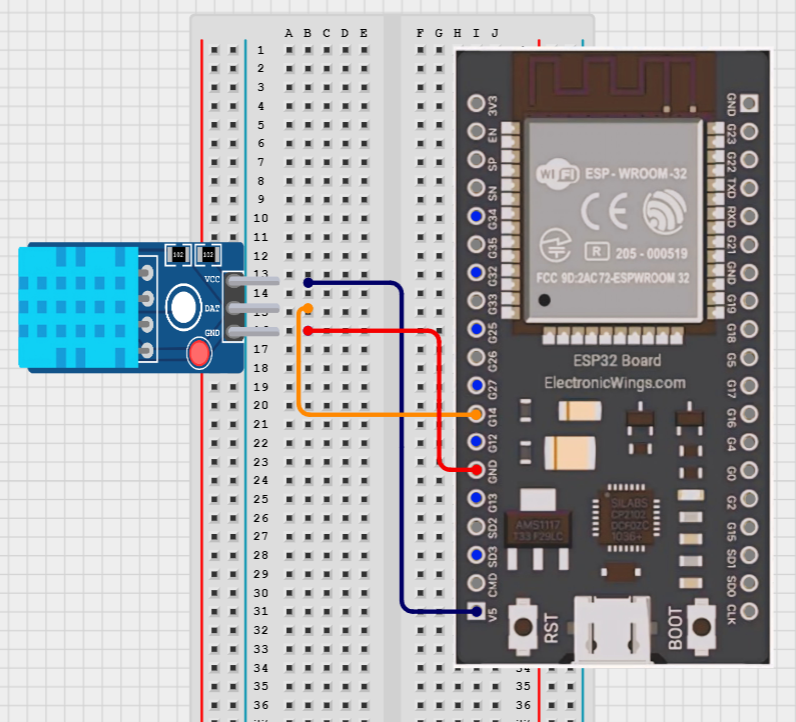
\includegraphics{circuit_image.png} } 
	 \vspace{10pt} 
	 \caption{Anhang: Schaltplan DHT11 (eigene Abbildung)}\label{anhang: Schaltplan} 
\end{figure}

\begin{figure}[H]
	 \centering 
	 \resizebox{\textwidth}{!}
	 { 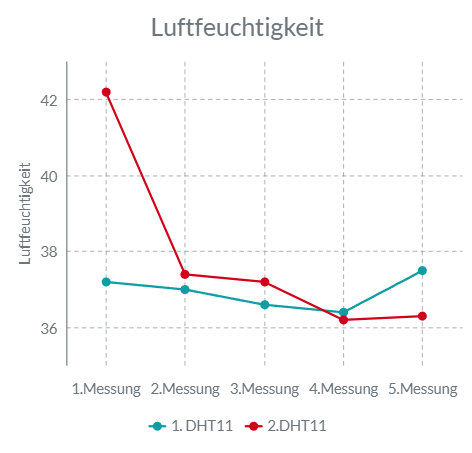
\includegraphics{Luftfeuchtigkeitsmessreihe.png} } 
	 \vspace{10pt} 
	 \caption{Anhang: Luftfeuchtigkeitsmessreihe}\label{anhang: Luftfeuchtigkeitsmessreihe} 
\end{figure}


\begin{figure}[H]
	 \centering 
	 \resizebox{\textwidth}{!}
	 { 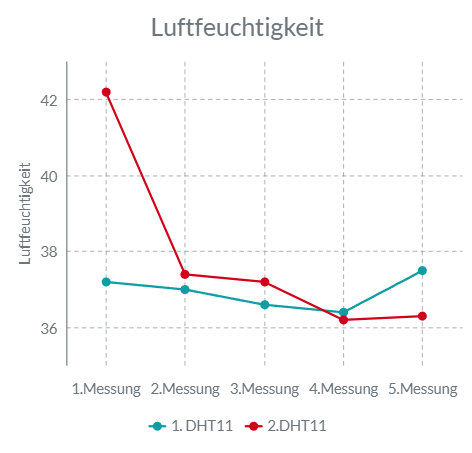
\includegraphics{Luftfeuchtigkeitsmessreihe.png} } 
	 \vspace{10pt} 
	 \caption{Anhang:Temperaturmessreihe}\label{anhang: Temperaturmessreihe} 
\end{figure}

\begin{figure}[H]
	 \centering 
	 \resizebox{\textwidth}{!}
	 { 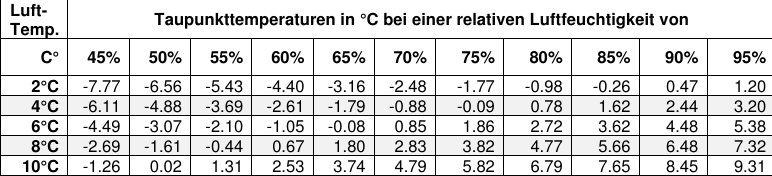
\includegraphics{ausschnitt_Taupunkttabelle.png} } 
	 \vspace{10pt} 
	 \caption{Anhang: Auschnitt aus der Taupunkttabelle \protect\citeM{d}{tauKor}{1}{1}}\label{anhang:Auschnitt_Taupunkttabelle} 
\end{figure}



\pagebreak
%\includepdf[pages=-,scale=.9,pagecommand={}]{Aufgabenstellung.pdf} % PDF um 10% verkleinert einbinden --> Kopf- und Fußzeile  werden so korrekt dargestellt. Die Option `pages' ermöglicht es, eine bestimmte Sequenz von Seiten (z.B. 2-10 oder `-' für alle Seiten) auszuwählen.
\pagebreak




	
\end{document}
